\chapter{Design of the Sensing System}
\label{ch:System}
%------------------------------------------------------------------------------

\section{System Overview}
\label{Sec:SystemOverview}

The \textit{ITrem2} sensing system consists of two sub-systems, the inertial measurement system and the vision system. 

\begin{figure*}[htbp!]
 \centering
 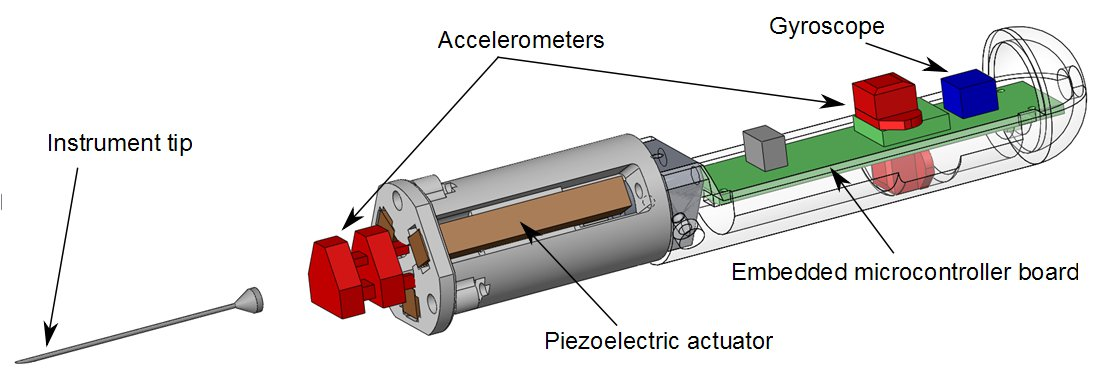
\includegraphics[width=1\textwidth]{./Fig/Fig_InstrumentComponents.jpg}
 \caption{\textit{ITrem2} schematic}
 \label{Fig_InstrumentComponents}
\end{figure*}

%--------------------------------------------------------------------------
%Include \usepackage{subcaption} to use subfigures
%\begin{figure}[H]
% \centering
%	\begin{subfigure}{0.45\textwidth}
%	\vspace{3cm}	
%	\centering
%	\includegraphics[width=\textwidth]{./Fig/SubFig1.pdf}
%	\caption{SubFig1 caption.}
%	\label{Fig:SubFig1}
%	\end{subfigure}
%	\hfill
%	\begin{subfigure}{0.4\textwidth}
%	\centering
%	\includegraphics[width=\textwidth]{./Fig/SubFig2.pdf}
%	\caption{SubFig2.}
%	\label{Fig:SubFig2}
%	\end{subfigure}
%	%\vskip\baselineskip
	
%	\begin{subfigure}{0.45\textwidth}	
%	\centering
%	\includegraphics[width=\textwidth]{./Fig/SubFig3.pdf}
%	\caption{SubFig3.}
%	\label{Fig:SubFig3}
%	\end{subfigure}
%	%\quad
%	\hfill
%	\begin{subfigure}{0.45\textwidth}
%	%\vspace{0.5cm}	
%	\centering
%	\includegraphics[width=\textwidth]{./Fig/SubFig4.pdf}
%	\caption{SubFig4.}
%	\label{Fig:SubFig4}
%	\end{subfigure}
%	\caption{Main caption}
%	\label{Fig:mainfig}
%\end{figure}
%--------------------------------------------------------------------------
